%% ABSTRACT %%
% In order to account for the model flexibility required by the multivariate
%     peaks-over-threshold scenario, a Dirichlet process mixture model using
%     the projection of independent gamma random variables onto the unit 
%     hypersphere under the $\mathcal{L}_p$ norm was developed.  This very
%     quickly presents computational issues, as the computational burden for
%     MCMC inference scales superlinearly with sample size, and will scale
%     either linearly or exponentially depending on choice of centering 
%     distribution. We propose an alternate approach, developing a 
%     variational Bayes approach for model inference.  We apply this model
%     to a dataset of simulations of storm surge; comprised of 4 thousand
%     observations at more than 21 million locations.

\subsection{SLOSH}]
\makenote{a lot of this is fluff.}
Storm surge inundation is localized flooding, defined as water height above
    ground level.  Its effect can be catastrophic.  Setting aside potential 
    for direct loss of life, 
    flooding can impose costly damage to property: inundation of homes and 
    businesses destroys possessions, and damages buildings through saturating 
    walls and eroding foundations.  Corrosion resulting from high--salinity 
    flooding can create more long--term  damage.\makenote{expand}\needcite  
    Flooding can damage vehicles, such that a single storm can force insurance 
    companies to declare large quantities of vehicles as total losses. 
    \makenote{expand}\needcite.  Flooding damages agriculture: beyond 
    destruction of currently growing or stored crops, or the drowning of 
    livestock, inundation by storm surge results in the ground absorbing salt, 
    affecting the production capacity of the field until abatement. Flooding can
    damage infrastructure: flooded roads can be washed out or have their 
    foundation damaged, flooded sewers and sewage treatment plants can release 
    their contents above ground imposing additional environmental costs.  
    Flooded power infrastructure, such as transformers can short out causing 
    additional damage. \citep{hutchings2021}.  Inundation can impose additional 
    burdens in the moment:  inundation negatively affects the quality of 
    emergency services, such as a hospital being rendered unable to intake 
    patients.  Sufficient flooding may even render a provider entirely out of 
    commission.

Sea, Lake, and Overland Surges from Hurricanes \citep{jelesnianski1992} is a 
    computer model developed by the National Weather Service to simulate storm 
    surge, and its associated inundation caused by hurricanes.   Given storm 
    characteristics, the model takes into account local topology, bathymetry, 
    and surge management devices such as levees, to generate a spatial field of 
    inundation---the maximum observed height of water above ground level 
    (or above normal water level for a data point in a body of water) for the 
    duration of the storm at a location.   These storm characteristics include 
    data pertaining to the eye of the storm when it made landfall---bearing, 
    velocity, latitude, minimum atmospheric pressure of the storm when it 
    made landfall, and projections of sea level rise over time.  A 
    \emph{simulation} from the model, for the basin we are analyzing, is a grid 
    containing \num{23119800} elements with a spatial resolution of 
    \num{0.001} degrees, or approximately 90 meters, \makenote{(verify)}, 
    covering an area extending from Virginia Beach, Virginia, to Long Island, 
    New York.  We have \num{4000} such simulations, produced by SLOSH from a 
    sample of storm characteristics.

\begin{figure}[ht]
    \centering
    \begin{minipage}{0.45\textwidth}
    \centering
    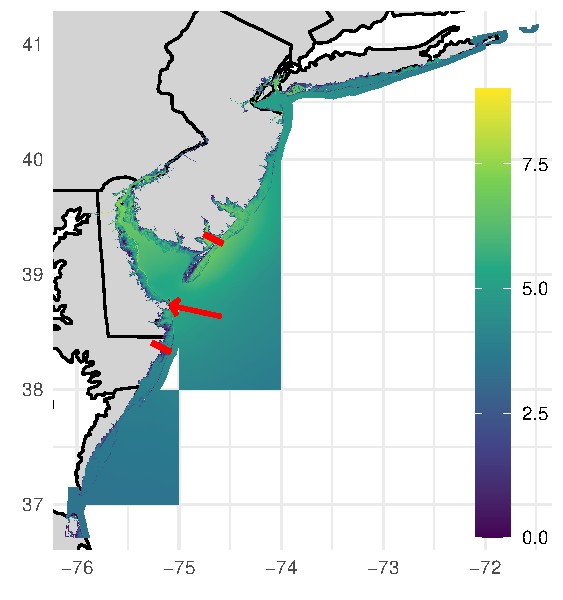
\includegraphics[width=0.99\linewidth]{./plots/slosh1run}
    \end{minipage}%
    \begin{minipage}{0.45\textwidth}
    \centering
    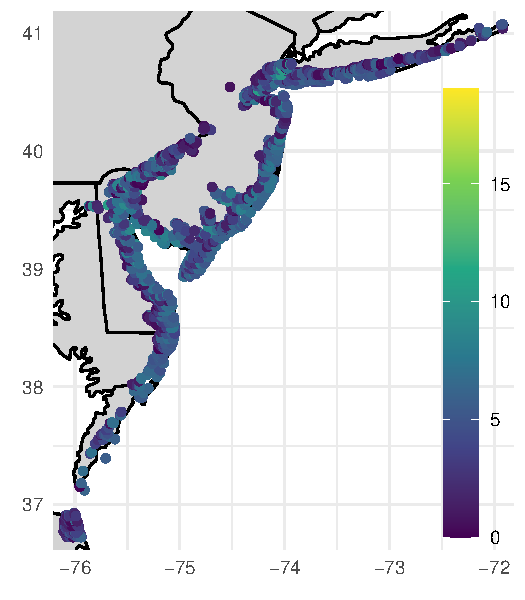
\includegraphics[width=0.99\linewidth]{./plots/sloshthreshold}
    \end{minipage}
    \caption{(Left) Grid output from one storm simulation in SLOSH.  (Right)  
        99th \%ile of storm surge simulations at selected points. 
        \makenote{Make single plot, with only 1 legend on right. Either that
        or maybe separate legends makes sense. Histogram on right next to legend would make most sense.  make points smaller, as well.\label{fig:sloshexplore}}}
\end{figure}

This paper analyzes SLOSH simulations under an extreme value framework, using a
    peaks-over-threshold model.  Extreme value theory is a branch of statistics
    that focuses on the tails of the distribution, low density regimes where,
    in this application, the \emph{worst} outcomes occur.  
    Figure~\ref{fig:sloshexplore} provides a visual depiction of the SLOSH 
    simulation data.  The left plot indicates the output of a single storm surge 
    simulation using the SLOSH model.   We should note that particularly high
    values of inundation are localized events, effectively not visible at this
    low scale. We should note here that a storm takes some time to occur, and 
    the recorded value is the maximum over the duration of the storm.  That 
    means that peak recorded values at two locations are not necessarily 
    simultaneous.
    On the right of Figure~\ref{fig:sloshexplore}, we have selected SLOSH grid 
    cells that are in the vicinity of physical features, or locations, of 
    interest.  Displayed are the 99th\makenote{subject to change} percentile 
    of inundation for SLOSH simulations at each of those physical features.
    We make clear now, that this analysis is primarily concerned with the
    inferring and applying the dependence structure between storm simulations
    that are in excess of this \emph{threshold} in at least one identified location.
    Our goal is then a consistent and performant model for multivariate extremes, 
    such that we can learn the dependence structure of extremes in the inundation field.
    
% Unfortunately, with respect to flooding in general, SLOSH provides only an 
%     incomplete picture.  It does not account for inundation due to rainfall or
%     rivers bursting their banks.

\makenote{I need to expound upon the necessity/applicability of extreme analysis
    to inundation.  Mention: importance of tails of the distribution, relevance of
    extremes to such analysis, }

The roadmap for our paper is as follows:  Section~\ref{ref:review} details the 
    background for the relevant modelling methods
    we will be using in this analysis.  In particular, Section~\ref{ref:evt} 
    provides an overview of extreme value theory, to the justification for 
    separating the magnitude of a multivariate extreme from its angular 
    component; Section~\ref{ref:pg} describes the process of creating an angular 
    distribution as well as introducing the model we use in our analysis; and 
    Section~\ref{ref:varbayes} introduces variational Bayesian methods, which we 
    can use to apply our model at large scale.  Section~\ref{ref:methodology} 
    \makenote{does something.  probably most of review should be moved here?  
    but none of that is new, only new thing is the particular variational model.}
    Section~\ref{ref:results} presents our analysis, first demonstrating the 
    efficacy of variational methods on simulated data as compared to MCMC, then
    presenting some interesting results. Finally, Section~\ref{ref:conclusion} 
    concludes.

% EOF 